\NeedsTeXFormat{LaTeX2e}

\documentclass[12pt]{article}
\usepackage[letterpaper,portrait, margin=1in]{geometry}
\usepackage{booktabs, pgfplots, bm, multirow, amsmath, wrapfig, gensymb, graphicx, amsfonts}
\pgfplotsset{width=11cm,compat=1.9}
\renewcommand{\arraystretch}{1.5}
\usepackage[colorlinks=true, allcolors=blue]{hyperref}
\usepackage{indentfirst}



\begin{document}

%%%%%%%%%%%%%%%%%%%%%%%%%%%%%%%%%%%%%%%%%%%%%%%%%%%%%%%%%%%%
%%% COVER PAGE - TO BE COPIED AT BEGINNING OF LAB REPORT %%%
%%%      PLEASE ALSO FILL OUT WITH YOUR INFORMATION      %%%
%%%%%%%%%%%%%%%%%%%%%%%%%%%%%%%%%%%%%%%%%%%%%%%%%%%%%%%%%%%%

\begin{titlepage}

       %\vspace*{.5cm}
        \begin{center}
        \textbf{\huge PH-291 Physics Lab} \\ 
        \textbf{\Large Professor Corn-Agostini} \\ 
        \textbf{\Large Fall 2022} \\ 
        \vspace*{.5cm}  
        \textbf{\large Lab \# 5: Diffraction \& Interference}
        \vspace{0.5cm}
        \end{center}
       
\noindent Your Name: Perla Berkovitz\\ \\
\noindent Your Lab Section:E\\ \\
\noindent Your Lab Instructor: Professor Corn-Agostini\\ \\
\noindent Your Lab Partner's Name: Sharon Sitt\\ \\
\noindent Read and sign Academic Integrity Statement:\\

\noindent {\em I hereby attest that I have not given or received any unauthorized assistance on this assignment.}

    \begin{center}
    \line(1,0){300} \\
    Sign here
    \end{center}

\noindent\textbf{\large Grading Rubric} \\ \\
\renewcommand{\arraystretch}{1.5}
%\large
\begin{tabular}{|l|c|r|l|} \hline
 {\bf CATEGORY} & {\bf POINTS} & {\bf GRADE}\\\hline 
Purpose & 2 & \\\hline
Data & 6 & \\\hline
Theory \& Calculations (includes Q1 and Q2) & 6 & \\\hline 
Results \& Analysis & 4 & \\\hline 
Conclusion  & 2 & \\\hline \hline 
{\em Total} & 20 & \\ \hline
\end{tabular}

\end{titlepage} 



\newpage
\tableofcontents
\newpage
\section{Purpose}
In this experiment, the wave nature of light will be analyzed by observing how a laser beam interacts with certain obstacles and openings.
First, the wavelength of the laser beam will be determined through the N-slit experiment.
The light will pass through a grating with 1,000 lines/mm onto a screen, and the location of the intensity maxima will then be used to calculate the wavelength. 
After determining this wavelength, a single slit is created using a Vernier caliper, and the wavelength is determined using the minima from the diffraction pattern generated by the slit.
The diameter of a human hair can then be determined using Babinet's principle which states that the diffraction pattern of a shape is identical to the diffraction pattern of a screen with the shape cut out of it. 
Here, the diffraction pattern of the hair is identical to the diffraction pattern of an opaque screen with a slit that has the same width as the hair. 
\newpage
\section{Data}
\begin{center}
    \begin{minipage}{.5\linewidth}
        \centering
        \begin{tabular}{|c | c|}
            \hline
            \textbf{Measurement} & \textbf{Thickness (mm)}  \\ \hline
            1 & 1.695 \\ 
            2 & 1.995 \\ 
            3 & 1.990  \\ 
            4 & 2.095 \\ 
            5 & 1.930 \\ 
            6 & 1.995 \\ \hline
            \multicolumn{2}{|c|}{\textbf{Instrumental Error:} 0.005 mm} \\
            \multicolumn{2}{|c|}{\textbf{Random Error:} 0.055 mm} \\
            \multicolumn{2}{|c|}{\textbf{Thickness:} $1.950\pm0.055$ mm} \\ \hline
        \end{tabular}
        \vspace{3mm}
        \\Table 1: Petri Dish Thickness
        \vspace{10mm}
    \end{minipage}%
    \begin{minipage}{.5\linewidth}
        \centering
        \begin{tabular}{|c | c|}
            \hline
            \textbf{Measurement} & \textbf{Thickness (mm)}  \\ \hline
            1 & 7.98 \\ 
            2 & 8.86 \\ 
            3 & 8.24  \\ 
            4 & 7.60 \\ 
            5 & 8.16 \\ 
            6 & 7.66 \\ \hline
            \multicolumn{2}{|c|}{\textbf{Instrumental Error:} 0.02 mm} \\
            \multicolumn{2}{|c|}{\textbf{Random Error:} 0.19 mm} \\
            \multicolumn{2}{|c|}{\textbf{Thickness:} $8.08\pm0.19$ mm} \\ \hline
        \end{tabular}
        \vspace{3mm}
        \\Table 2: Ring Diameter Without Liquid
        \vspace{10mm}
    \end{minipage} 
    \begin{tabular}{|c|c|}
        \hline
        \textbf{Measurement} & \textbf{Diameter (mm)} \\ \hline
        1 & 19.68 \\ 
        2 & 19.60 \\ 
        3 & 19.58 \\ 
        4 & 19.58 \\ 
        5 & 19.56 \\ 
        6 & 19.62 \\ \hline
        \multicolumn{2}{|c|}{\textbf{Instrumental Error:} 0.02 mm} \\
        \multicolumn{2}{|c|}{\textbf{Random Error:} 0.017 mm} \\
        \multicolumn{2}{|c|}{\textbf{Thickness:} $19.60\pm0.02$ mm} \\ 
        \hline
    \end{tabular}
    \vspace{3mm}
    \\Table 3: Ring Diameter With Liquid
    \begin{tabular}{|c|c c|}
    \hline
        \textbf{Measurement} & \textbf{Incident Angle} & \textbf{Refracted Angle} \\ \hline
        1 & $50.0\degree$ & $28.0\degree$ \\ 
        2 & $28.0\degree$ & $38.0\degree$ \\ 
        3 & $36.0\degree$ & $20.0\degree$ \\ 
        4 & $17.0\degree$ & $40.0\degree$ \\ 
        5 & $43.0\degree$ & $27.0\degree$ \\ 
        6 & $28.0\degree$ & $39.0\degree$ \\ \hline
        \multicolumn{3}{|c|}{\textbf{Instrumental Error:} $0.5\degree$} \\ \hline
    \end{tabular}
    \vspace{3mm}
    \\Table 4: Snell's Law
\end{center}
\newpage
\section{Calculations}
\subsection*{Part A: Determination of a Laser's Wavelength}
\noindent \textbf{1. Intensity due to the interference of $\bm{N}$ sources}\[I(\delta)=I_0\left[\frac{\sin(\frac{N\delta}{2})}{\sin(\frac{\delta}{2})}\right]^2 \quad \text{where} \quad \delta=\frac{2\pi}{\lambda}d\sin\theta\]
Here, $d$ is the distance between slits, $\lambda$ is the wavelength of light, and $\theta$ is the angle between the center of the incident beam of light and the point of interest on the screen. 
In our experiment, we were interested in the peaks of the interference pattern.\\
\textbf{1.1 Determining $\bm{\theta}$}\[\tan\theta=\frac{x_m}{D}\Rightarrow\theta=\arctan\frac{x_m}{D} \quad m=0,\pm1\pm2,\dots\]
Where $D$ is the distance between the grating and the screen, and $x_m$ represents the distance between the center and each of the principal maxima.
\subsubsection*{Error Propagation:}
    \noindent\textbf{1.1.1 Partial Derivative of Eq. 1.1 w.r.t $\bm{D}$}\[\frac{\partial\theta}{\partial D}=\frac{-x_m}{D^2+x_m^2}\]
    \textbf{1.1.2 Partial Derivative of Eq 1.1 w.r.t $\bm{x_m}$}\[\frac{\partial\theta}{\partial x_m}=\frac{D}{x_m^2+D^2}\]
    Using the above partial derivatives, we can calculate the total error associated with $\theta.$ Because $D$ and $x_m$ are dependant variables, we use the following equation to compute the total error.\\
    \textbf{1.1.3 Total Error Associated with $\bm{\theta}$}\[\delta\theta=\left|\frac{\partial\theta}{\partial D}\delta D\right|+\left|\frac{\partial\theta}{\partial x_m}\delta x_m\right|\]
\noindent\textbf{2. Principal Maxima Locations}\[\sin\theta=\frac{m\lambda}{d} \quad m=0,\pm1,\pm2,\dots\]
    Here $m$ refers to each of the principal maxima. For example in Table 1, the $x_{+1}$ column refers to the $m=1$ maxima
\subsubsection*{Error Propagation:}
    \noindent\textbf{2.1 Partial Derivative of Eq. 2 w.r.t $\bm d$}\[\frac{\partial\lambda}{\partial d}=\frac{\sin\theta}{m}\]
    \textbf{2.2 Partial Derivative of Eq. 2 w.r.t $\bm \theta$} \[\frac{\partial f}{\partial \theta}=\frac{d}{m}\cos\theta\]
    \textbf{2.3 Partial Derivative of Eq. 2 w.r.t $\bm m$} \[\frac{\partial f}{\partial m}=\frac{-d\sin\theta}{m^2}\]
    Each of these partial derivatives are used in the final calculation of the total error associated with $\lambda.$ These variables are independent, which allows us to use the following equation to calculate the total error.\\
    \textbf{2.4 Total Error Associated with the Wavelength $\bm{(\lambda)}$}\[\delta \lambda =\sqrt{\left(\frac{\partial \lambda}{\partial d}\delta d\right)^2+\left(\frac{\partial \lambda}{\partial \theta}\delta \theta\right)^2+\left(\frac{\partial \lambda}{\partial m}\delta m\right)^2}\]
    In our experiment, $m$ represents the number of the principal maxima, so there is no error associated with it. The total error associated with the mean values were calculated (shown in the Results section). This provides our final error associated with $\lambda$.\\
\subsection*{Part B: Single Slit Diffraction}
    \noindent\textbf{3. Intensity due to a Single Slit}\[I(\beta)=I_0\left(\frac{\sin\beta}{\beta}\right)^2\quad where \quad \beta=\frac{\pi}{\lambda}a\sin\theta\]
    Here, $a$ is the width of the slit and $\lambda$ and $\theta$ are as given in Equation 1.\\
\textbf{4. Minima of the Diffraction Pattern Locations} \[\sin\theta=\frac{p\lambda}{a} \quad p=0,\pm1,\pm2,\dots\]
This equation matches with Equation 2, where $a$ is analogous to $d$ and $p$ is analogous to $m$. When determining the error in calculating the wavelengths for a single slit, the Standard Deviation of the Mean is calculated.\\    
\textbf{4.1 Error Calculation: Standard Deviation of the Mean (SDOM)}\[\sigma_{\bar{x}}=\frac{S_x}{\sqrt{N}}\]
    Where $S_x$ is the standard deviation of the data and $N$ is the number of data points. For our single slit wavelength calculations, 12 values for the wavelength were calculated, meaning $N=12$.
\subsection*{Determination of a Hair's Thickness}
\noindent\textbf{5. Slit Thickness}\[a=\frac{\lambda p}{\sin\theta}\]
Rearranging Equation 4 to solve for the slit width gives this equation, which allows us to calculate the thickness of the hair, given the value of $\lambda$. 
To determine the error of the hair's thickness, the SDOM was calculated, using Equation 4.1, where $N=6$, since there were thickness values for the first, second, and third order peaks. 
\newpage
\section{Results}
\begin{center}
    \centering
    \begin{tabular}{|c|c|c|c|}
    \hline
        $n_\text{glass}$ & $\frac{\partial n_\text{glass}}{\partial t}$ & $\frac{\partial n_\text{glass}}{\partial d}$ & Error of $n_\text{glass}$ \\ \hline
        1.39 & 0.34 & -0.08 & 0.08 \\ \hline
        \multicolumn{4}{|c|}{$\bm{n_\textbf{glass}: 1.39\pm0.08}$}\\\hline
    \end{tabular}
    \vspace{3mm}
    \\ Table 5: $n_\text{glass}$ Final Value by Pfund's Method\\
    \vspace{5mm}
    \centering
    \begin{tabular}{|c|c|c|c|c|c|}
    \hline
        $n_\text{liquid}$ & $\frac{\partial n_\text{liquid}}{\partial t}$ & $\frac{\partial n_\text{liquid}}{\partial d}$ & $\frac{\partial n_\text{liquid}}{\partial n_{\text{glass}}}$ & Error of $n_\text{glass}$ & Error of $n_\text{liquid}$ \\ \hline
        1.29 & -0.09 & 0.009 & 0.93 & 0.08 & 0.26 \\ \hline
        \multicolumn{6}{|c|}{$\bm{n_\textbf{liquid}: 1.29\pm0.26}$}\\\hline
    \end{tabular} 
    \vspace{3mm}
    \\ Table 6: $n_\text{liquid}$ Final Value by Pfund's Method\\
    \vspace{5mm} 
    \centering
    \begin{tabular}{|c|c|c|c|}
    \hline
        $n_\text{liquid}$ & $\frac{\partial n_\text{liquid}}{\partial \theta_1}$ & $\frac{\partial n_\text{liquid}}{\partial \theta_2}$  & Error of $n_\text{liquid}$ \\ \hline
        1.62 & 1.88 & -3.82 & 0.04  \\ \hline
        \multicolumn{4}{|c|}{$\bm{n_\textbf{liquid}: 1.62\pm0.04}$}\\\hline
    \end{tabular} 
    \vspace{3mm}
    \\ Table 7: $n_\text{liquid}$ Final Value by Snell's Law\\
    \vspace{5mm}
    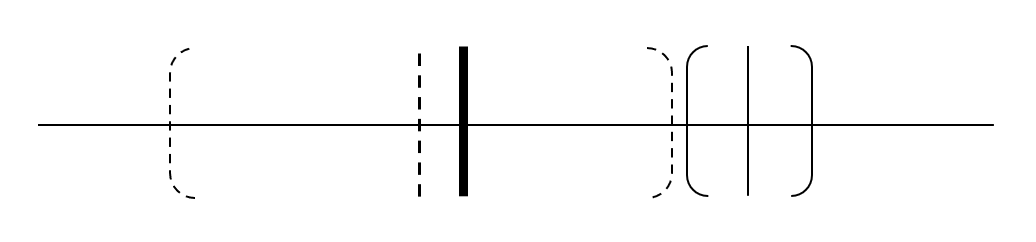
\includegraphics[scale=0.5]{number line.png}\\
    Dashed = Method 1 (Pfund's Method)\\
    Solid = Method 2 (Snell's Law)\\
    Bold = Accepted Value \\
    Figure 1: Number Line Indicating Error Bounds and Accepted Values   
\end{center}
Using Figure 1, we can see that while the index of refraction calculated via Pfund's Method had a greater error, it was closer to the accepted value of the index of refraction of water, which is 1.33. The accepted index of refraction lies within the error bounds of the Pfund's Method calculation. Snell's method provided an index of refraction of $1.62\pm0.04$ which does not agree with the accepted value. This can mainly be attributed to human error in measuring the incident and refracted angles. When measuring our angles, we misread our protractor as having increments at every $1\degree$, as opposed to every $0.5\degree$. This provided us with an instrumental error of $0.5\degree$, as opposed to $0.25\degree$.
\\\indent The error introduced in Pfund's Method stems from multiple areas. Firstly, the petri dish may not have had a uniform thickness, providing different thickness readings on the micrometer. Then, the laser may not have been pointed perfectly vertically. Pfund's method relies on the laser making an angle of $\frac{\pi}{2}$ with the horizontal. Lastly, error is introduced in measuring each of the rings. The method of measuring required eyeballing where the ring lined up on the polar grid and then measuring the polar grid on a separate piece of paper. Measurements were taken using a pair of vernier calipers, which have pointed ends where the measurements are taken. These tended to make indentations in the polar grid paper which the calipers would slide into when taking other measurements.\\
\indent The second method using Snell's Law had less error associated with the final index of refraction relative to the value found by Pfund's Method. The calculated index of refraction is $1.62\pm0.04$. While tracing the petri dish onto our surface, the polar grid on the bottom of the dish caused us to trace a larger circle than the diameter of the petri dish. Then, when placing the pins along the path of the laser, the laser may have been nudged out of position. This would affect the accuracy of our measured angles. The center of the circle may also have been misplaced, as it is found using the perpendicular bisectors of two cords. These perpendicular bisectors may not have been exactly perpendicular. This would affect the measurements taken for our angles, and in turn affect our index of refraction.
\newpage
\section{Conclusion}
The wavelength of a red laser beam was calculated using an N-slit interference pattern to be  $(6.68\pm0.04)\times10^{-5}$ cm. 
Using a single slit interference pattern, with various slit widths, the wavelength was determined to be $(6.3\pm 0.3)\times10^{-5}$ cm.
Both of these wavelength values lie within the expected wavelength of red light, which varies between 630 nm and 670 nm.
Based on the calculated wavelength of the single slit diffraction, the thickness of a human hair was determined using Babinet's principle to be $0.0087 \pm 0.0006$ cm. 
This thickness lies within the accepted thickness of a hair, which varies between $15 \mu$m and $181 \mu$m based on the type of hair used.
Although the experimental values of wavelength and hair thickness lie within their accepted ranges, there were many sources of error within the experiment. 
Further experimental measurements can provide greater accuracy for the wavelength and thickness calculations.
Once the sources of error are reduced, a more accurate value can be calculated via both the N-slit and single slit diffraction. 
\newpage
\section{Questions}
\subsection*{1. Explain why $(\sin\theta=\frac{m\lambda}{d}, m\in\mathbb{Z})$ is so. You will have to take the appropriate limits for Equation 1 $\left(I(\delta)=I_0\left[\frac{\sin\frac{N\delta}{2}}{\sin\frac{\delta}{2}}\right]^2, \delta= \frac{2\pi}{\lambda}d\sin\theta\right)$}
\noindent This equation comes from the limit of the maxima of the intensity for an N-slit diffraction pattern, given in the above equation.
\[\lim_{\delta\rightarrow\infty}\frac{\sin(N\delta)}{\sin\delta}=\frac{0}{0}\]
Using L'Hopital's Rule
\[\lim_{\delta\rightarrow\infty}\frac{N\cos(N\delta)}{\cos\delta}=\frac{-N}{-1}=N\]
\[I(\delta)\text{at maxima } (\pi,2\pi,\dots)=I_0N^2\]
\[\delta=\pi,2\pi,\dots,m\pi,  m\in \mathbb{Z}\]
\[\sin\theta=\frac{\delta\lambda}{2\pi d}=\frac{m\pi\lambda}{2\pi d}=\frac{m\lambda}{d} \quad m\in\mathbb{Z}\quad\text{as desired.}\]
\subsection*{2. Explain how we arrive at $\left(\sin\theta=\frac{p\lambda}{a}, p=\pm1,\pm2,\dots\right)$ from Equation 3 $\left(I(\beta)=I_0\left(\frac{\sin\beta}{\beta}\right)^2 \right)$}
\noindent This equation comes from the minima of the intensity for a single slit diffraction pattern, which occurs when $\frac{\pi}{\lambda}a\sin\theta=\pi,2\pi,\dots, m\pi,\quad m\in\mathbb{Z}$.
\[\frac{\pi}{\lambda}a\sin\theta=m\pi\]
\[\sin\theta=\frac{m\pi\lambda}{\pi a}=\frac{m\lambda}{a}\quad\text{as desired.}\]
\end{document}